\documentclass{aitthesis}
\usepackage{amsmath,amssymb}

\usepackage{multirow}
\usepackage{graphicx}
\usepackage{subfig}
\usepackage[justification=centering]{caption}

\usepackage{graphicx}
\usepackage{caption}
\captionsetup[figure]{labelsep=colon, justification=centering}

% This command enforces the "Figure X: Caption" single-line format and centering
% This command enforces the "Figure X: Caption" single-line format and centering
\captionsetup{format=plain, labelsep=colon, justification=centering}
\captionsetup[table]{labelsep=colon, justification=centering}

\usepackage{listings}
\lstset{
  basicstyle=\ttfamily\small,
  breaklines=true,
  breakatwhitespace=true,
  columns=flexible,
  frame=single,
  numbers=left,
  numberstyle=\tiny,
  showstringspaces=false
}

\bibliographystyle{apacite}

\begin{document}

\pagenumbering{roman}
\addtocontents{toc}{~\hfill\textbf{Page}\par} %This adds the word Page on top of the table of content

\setcounter{page}{1}
\thispagestyle{empty} 

\begin{center}
{ 
  \large{\bf Water Level Prediction at Krungthep Bridge (CPY015 Station)}
}

\vskip 3em
by
\vskip 3em
Dechathon Niamsaard\\
Zwe Yu Ya Kyaw Zin Oo
\vskip 3em
A Project Report Submitted in Partial Fulfillment of the
Requirements for the Course\\ Computer Programming for Data Science and Artificial Intelligence\\ 
in Data Science and Artificial Intelligence

%	\vskip 5em
\vskip 3em
{
  \begin{center}
    \begin{tabular}{rl}
      \\[-1em]
      Instructor: & Asst.\ Prof.\ Chantri Polprasert \\
	    \\
	    \\
      Nationality:     & Thai, Myanmar \\
      Previous Degree: & Bachelor of Engineering, Bachelor of Science \\
                       & \\
                       & \\
      \\
      \\
    \end{tabular}
  \end{center}

  \vskip 1em
}
\vfill
\end{center}
\begin{center}
  Asian Institute of Technology\\ School of Engineering
                  and Technology\\ Thailand\\ December 2025
\end{center}
\vfill

\begin{center}
    \large{\bf AUTHORS' DECLARATION}
\end{center}

We, Dechathon Niamsaard and Zwe Yu Ya Kyaw zin Oo, declare that the research work carried out for this project was in accordance with the regulations of the Asian Institute of Technology. The work presented in it are our own and has been generated by us as the result of our own original research, and if external sources were used, such sources have been cited. It is original and has not been submitted to any other institution to obtain another degree or qualification. This is a true copy of the report including final revisions.

Date: December 2025

Names: 
\begin{itemize}
    \item Dechathon Niamsaard
    \item Zwe Yu Ya Kyaw zin Oo
\end{itemize}

\vspace{2em}

\phantomsection
\addcontentsline{toc}{chapter}{\bf ACKNOWLEDGEMENTS}
\begin{center}
    \large{\bf ACKNOWLEDGEMENTS}
\end{center}

We would like to express our sincere gratitude to our instructor, Asst. Prof. Chantri Polprasert, for his guidance and support throughout this project. We also thank the Asian Institute of Technology for providing the resources and environment necessary for this study. Special thanks to the Hydro-Informatics Institute (HII) and Open-Meteo for providing the essential data used in this research.

\phantomsection
\addcontentsline{toc}{chapter}{\bf ABSTRACT}

\begin{center}
    \large{\bf ABSTRACT}
\end{center}

\noindent
This project develops a machine learning and deep learning-based flood early warning system for Thailand by predicting river water levels 24 hours in advance using a merged hydro-meteorological dataset (Station CPY015) along the Chao Phraya River. By integrating historical water level data, meteorological variables from Open-Meteo, and river discharge signals, the system applies both classical machine learning models and an end-to-end LSTM network. The proposed LSTM model achieves a Mean Absolute Error (MAE) of 0.0989 m and an $R^2$ score of 0.9610, significantly outperforming baseline methods. The system generates continuous forecasts and risk assessments to support early warning and flood management decisions.

\vspace{0.5em}
\noindent \textbf{Index Terms}---Water Level Prediction, Flood Forecasting, LSTM, Early Warning System, Real-Time Monitoring.
\include{contents}
\include{loft}

\pagestyle{plain}
\pagenumbering{arabic}

\chapter{Introduction} 

\section{Introduction to Flood Prediction and Early Warning System}

Flooding is one of the most common natural disasters in the world and has consistently posed major threats to human lives, infrastructure, and national economies. In Thailand, flood events have repeatedly caused widespread damage, particularly in low-lying river basins and densely populated provinces. With climate change intensifying rainfall variability and increasing the frequency of extreme weather, the impact of floods has become more challenging to predict and manage. Therefore, early warning systems and predictive models are increasingly essential for mitigating risks and supporting timely decision-making.

Flood prediction and early warning systems aim to provide actionable forecasts based on hydrological and meteorological conditions, enabling communities and responsible agencies to prepare for possible flood events. Traditional forecasting systems often rely heavily on physical hydrological models or manual monitoring and may not provide localized or timely predictions in all regions. With improvements in data availability and computational power, machine learning has emerged as a viable alternative, allowing systems to learn from historical patterns and make short-term water level predictions with improved responsiveness. However, effective data handling and proper predictive modeling are required.

\begin{figure}[htbp]
    \centering
    % Ensure your file path is correct
    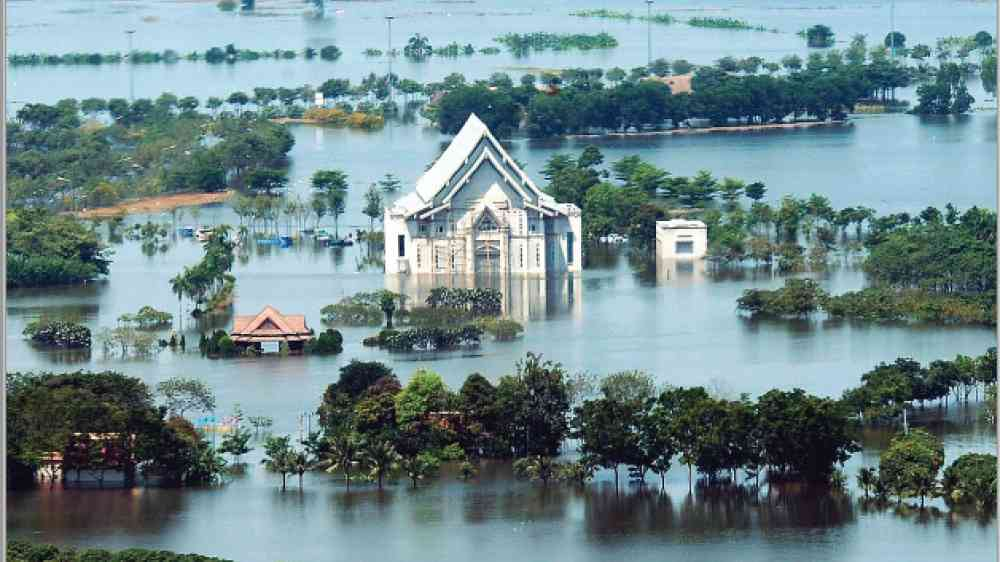
\includegraphics[width=0.95\textwidth]{figures/figure1.jpg}
    \caption{2011 Thailand's Flood.}
    \label{fig:complete_grid}
\end{figure}

\section{Global perspective of Flood}

According to the World Meteorological Organization (WMO, 2025)\cite{wmo2025floods}, floods account for nearly 40 percent of all natural disasters worldwide and have been the most widespread natural hazard globally. From flash floods in rural areas to large-scale river floods, no region remains unaffected. The number of flood-related events has increased significantly over the past decades, driven largely by rising global temperatures and erratic rainfall patterns. Moreover, rapid urbanization and land-use changes have further worsened flood risks by reducing natural drainage and increasing surface runoff. These conditions emphasize the urgent need for robust flood forecasting solutions and scalable early warning mechanisms, especially as climate change continues to deviate global weather patterns.

\section{Local Perspective of Flood (Thailand)}

Since Thailand is also regarded as one of the most vulnerable countries to climate-related disasters in Southeast Asia, floods remain one of the most frequent and devastating threats to humans. As stated by (Nation, 2024)\cite{thenation2024ongoing}, nearly 26,000 households in both the Northern and Eastern regions of Thailand are still overwhelmed by flooding, and 46 people have drowned to death, while 24 have sustained injuries as of the date 16th August 2025.

\begin{figure}[htbp]
    \centering
    
\includegraphics[width=\linewidth]{figures/figure2.jpg}
    \caption{Impact of Thailand’s flood in 2025.}
    \label{fig:impact_thailand_flood}
\end{figure}

\section{Why Do We Do This Project?}

\begin{table}[htbp]
    \centering
    \caption{Project Motivation and Rationale}
    \label{tab:motivation}
    \begin{tabular}{l p{10cm}}
        \hline
        \textbf{Motivation} & \textbf{Description} \\
        \hline
        \textbf{Public Safety} & Early flood warnings save lives and protect property. \\
        \textbf{Critical Location} & Krungthep Bridge is a key monitoring point in Bangkok. \\
        \textbf{Data Availability} & 6+ years of hourly water level data (2019-2025). \\
        \textbf{Technical Challenge} & Complex temporal patterns require advanced ML approaches. \\
        \textbf{Real-world Application} & Results can be deployed for actual flood monitoring. \\
        \hline
    \end{tabular}
\end{table}

\section{Problem Statement}

The problem we aim to solve is: ``How can we build a predictive system that accurately forecasts water levels and provides early warnings to reduce the losses caused by floods in Thailand?''

The proposed solution is a data-driven flood prediction and early warning system using supervised machine learning to forecast in the following manner.

\vspace{0.5em}
\noindent \textbf{Inputs:}
\begin{itemize}
    \item Water level (hourly)
    \item Meteorological data (temperature, wind, humidity, pressure, rainfall)
    \item River discharge
    \item Temporal features (hour, month, cyclical encoding)
\end{itemize}

\noindent \textbf{Outputs:}
\begin{itemize}
    \item 24-hour future water-level forecasts (continuous)
    \item Risk levels (categorical) based on bank capacity thresholds
    \item Used for Thailand’s river monitoring and forecasting
    \item Uses real-time weather data from Open-Meteo
\end{itemize}

\subsection{Possible Users}
\begin{enumerate}
    \item \textbf{Various agencies:} Infrastructure managers, including municipalities, as well as the Hydro-informatics Institute (HII).
    \item \textbf{Emergency responders:} Need precise flood forecasts to facilitate evacuation plans.
    \item \textbf{Farmers and communities who live in flood-prone areas:} Rely on early warnings to safeguard crops, livestock, and property.
\end{enumerate}
\setlength{\footskip}{8mm}

\chapter{Literature Review}
\label{ch:literature-review}

\section{Flood Prediction and Warning Systems}

The \textbf{Hydro-Informatics Institute (HII)} of Thailand developed comprehensive flood prediction and warning systems for urban areas in 2020. Their work established foundational frameworks for integrating hydrological models with real-time monitoring systems, enabling more effective flood management across Thai cities. This research demonstrated the importance of combining multiple data sources for improved prediction accuracy \cite{hii2024flood}.

\section{AI-Based Flood Monitoring}

\textbf{One More Link (2025)} introduced CCTV AI-based smart flood monitoring and early warning systems. This innovative approach uses computer vision and artificial intelligence to detect flood conditions from camera feeds, providing real-time alerts. Their work highlights the potential of AI technologies for automated flood detection and complements our water level prediction approach by providing visual verification of predictions \cite{onemorelink2025cctv}.

\section{Global Early Warning Systems}

The \textbf{World Meteorological Organization (WMO)} leads global efforts in developing comprehensive Early Warning Systems through their "Early Warnings for All" initiative. This framework emphasizes multi-hazard early warning, risk knowledge, monitoring and forecasting services, and communication systems. Our project aligns with WMO's recommended approaches by integrating meteorological data with hydrological measurements for improved forecast accuracy \cite{wmo2024ews}.

\section{Machine Learning for Water Level Forecasting}

\textbf{Fu et al. (2024)} demonstrated the effectiveness of combining machine learning with Ensemble Kalman Filtering for water level forecasting in Taiwan's Danshui River System. Their research showed that hybrid approaches combining data-driven ML models with statistical filtering techniques can achieve superior performance compared to standalone methods. This work informed our decision to compare multiple ML approaches including ensemble methods (XGBoost, LightGBM) and deep learning (LSTM) \cite{fu2024water}.

\section{Synthesis and Gaps}

While existing systems like HII's rely heavily on physical models or manual monitoring, and others like One More Link focus on visual detection, there is a gap in localized, data-driven predictive modeling that provides sufficient lead time (24 hours) for evacuation. Our work addresses this by developing a station-specific LSTM model that integrates multi-source data (water level, weather, discharge) to provide accurate, continuous future water level predictions with explicit risk classifications.

\setlength{\footskip}{8mm}

\chapter{Methodology}
\label{ch:methodology}

\section{Data Set}

\subsection{Description}
The primary dataset used in this project is a merged hydro-meteorological time series created by integrating three distinct sources:

\begin{itemize}
    \item \textbf{1. Water Level Data (Station CPY015)}

    This dataset\cite{hiiwaterlevel} originates from the \textbf{Thai Water Reporting System (Hydro-Informatics Institute)} and contains hourly water level measurements in meters above Mean Sea Level (m.MSL). Station CPY015 is located at latitude 13.7361 and longitude 100.5464, with reference values including Ground Level (1.951 m.MSL), Bank Level (2.161 m.MSL), and Bed Level (-15.70 m.MSL).

    \item \textbf{2. Meteorological Data (Open-Meteo)}

    To enrich the hydrological records, historical weather data were retrieved through the Open-Meteo archive API\cite{openmeteo} and provides hourly observations for the following meteorological variables:
    \begin{itemize}
        \item \texttt{temperature\_2m}
        \item \texttt{rain}
        \item \texttt{showers}
        \item \texttt{relative\_humidity\_2m}
        \item \texttt{pressure\_msl}
        \item \texttt{wind\_speed\_10m}
        \item \texttt{et0\_fao\_evapotranspiration}
    \end{itemize}

    \item \textbf{3. River Discharge Data (Open-Meteo Flood API)}

    Upstream flow conditions were captured using the Open-Meteo Flood API, which provides modeled river discharge estimates in $m^3/s$. Discharge values were sampled near the station location and merged with water level and weather data through time-based interpolation to align with the prediction timeline.
\end{itemize}

\subsection{Key Feature Groups}
\begin{itemize}
    \item \textbf{Hydrological Features:}
    Includes \texttt{river\_discharge}, \texttt{water\_level}, and derived lag features at 1, 2, 3, 6, 12, and 24 hours.

    \item \textbf{Rolling Statistics:}
    To capture recent trends and variability, rolling \texttt{mean}, \texttt{std}, \texttt{min}, and \texttt{max} statistics were calculated over windows of 6, 12, and 24 hours.

    \item \textbf{Difference Features:}
    Rate of change features were generated by calculating the difference between the current water level and values from 1 hour and 24 hours prior.

    \item \textbf{Temporal Features:}
    To capture cyclical patterns (daily tides and seasonal monsoons), temporal values (hour of day, month) were encoded using sine and cosine transformations.
\end{itemize}

\textbf{Target Labels:}
\begin{itemize}
    \item \textbf{Primary Output:} \texttt{water\_level} (continuous value in m.MSL) predicted 24 hours into the future.
    \item \textbf{Secondary Output:} Risk classification (Low, Medium, High, Critical) as detailed in Section \ref{sec:risk_standards}.
\end{itemize}

\subsection{Risk Classification Standards}
\label{sec:risk_standards}
To provide actionable early warnings, predicted water levels are mapped to risk categories based on the station's hydraulic capacity. This classification logic is adapted from the \textbf{ThaiWater} reporting standards (Hydro-Informatics Institute)\cite{thaiwater_wl}.

For Station CPY015 (Krungthep Bridge), the risk level is determined by the percentage of effective bank capacity utilized:
\begin{equation}
    \text{Capacity \%} = \frac{\text{Water Level} - \text{Bed Level}}{\text{Bank Level} - \text{Bed Level}} \times 100
\end{equation}
where:
\begin{itemize}
    \item \textbf{Bank Level:} 2.161 m.MSL (Critical overflow point)
    \item \textbf{Bed Level:} -15.70 m.MSL (River bottom)
\end{itemize}

The resulting percentages are classified as follows:
\begin{itemize}
    \item \textbf{Critical ($\ge 90\%$):} Imminent flood danger. Water level is near or above bank capacity.
    \item \textbf{High Risk ($70-90\%$):} Warning level. Significant rise requiring monitoring.
    \item \textbf{Medium Risk ($30-70\%$):} Normal to elevated levels.
    \item \textbf{Low Risk ($< 30\%$):} Safe operating levels.
\end{itemize}

\section{Data Acquisition}

The dataset for this study was constructed by combining in-situ river water level measurements with meteorological and discharge estimates into a unified hourly time series. Water level records were collected from Station CPY015 through the Hydro-Informatics Institute platform, while historical weather data and discharge estimates were retrieved using Open-Meteo APIs. All sources were aligned to a consistent hourly frequency, spanning January 2019 to May 2025, resulting in over 56,000 hourly observations.

\section{Exploratory Data Analysis (EDA)}

The final merged dataset consists of 56,232 hourly records spanning over six years. Comprehensive analysis reveals critical hydrological patterns that inform our modeling strategy.

\subsection{Temporal Patterns and Seasonality}
The water level time series (Figure \ref{fig:water_level_ts}) exhibits distinct seasonal cyclicity driven by Thailand's monsoon seasons. Annual peaks consistently occur between September and November, corresponding to the late rainy season and high river discharge periods. Conversely, dry seasons (December to April) show stable, lower water levels. These strong seasonal components confirm the necessity of including time-based features (month, day of year) and long-term lag features to capture annual periodicity.

\begin{figure}[htbp]
    \centering
    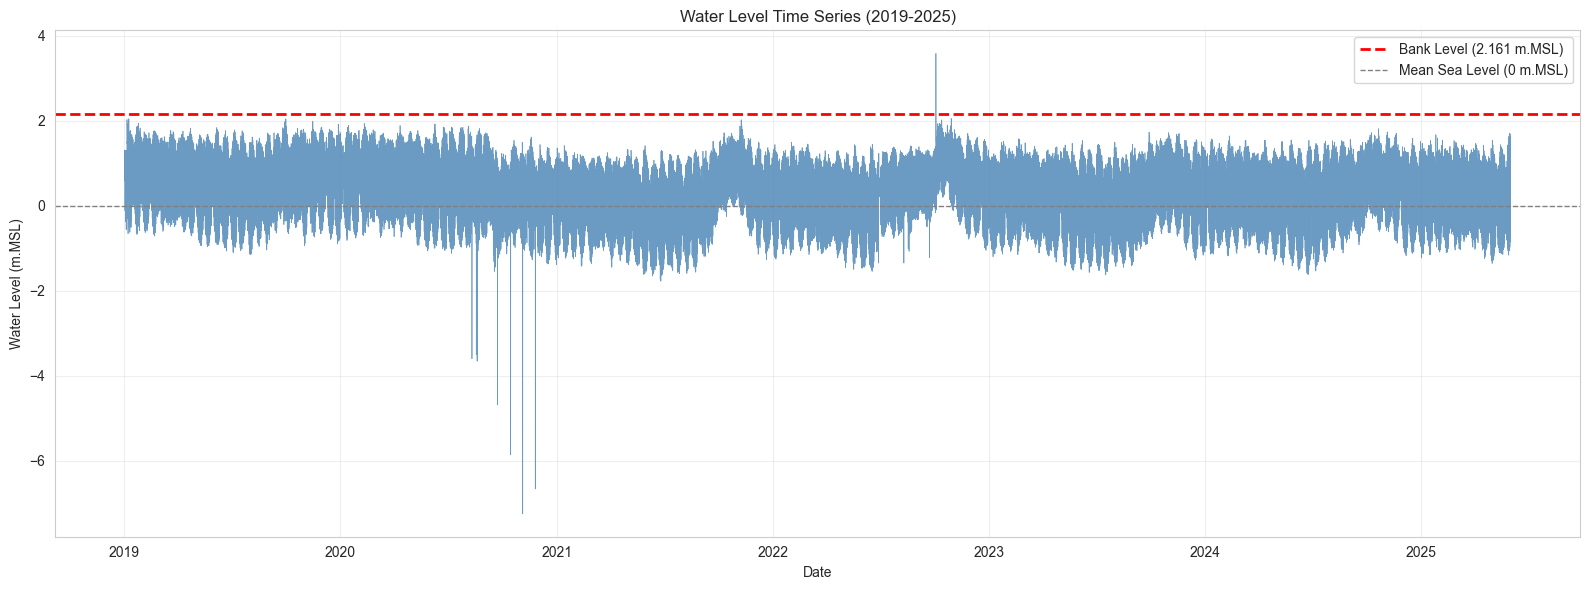
\includegraphics[width=0.9\textwidth]{figures/water_level_2019_2025.png}
    \caption{Water Level Time Series (2019-2025).}
    \label{fig:water_level_ts}
\end{figure}

\subsection{Feature Relationships}
Correlation analysis (Figure \ref{fig:correlation_matrix}) quantifies the drivers of water level changes. We observed a strong positive correlation ($r=0.85$) between water level and \texttt{river\_discharge}, confirming that upstream flow is the primary physical driver. Rainfall variables show moderate positive correlation ($r \approx 0.45$), acting as secondary contributors. The Pair Plot (Figure \ref{fig:pair_plot}) further reveals that these relationships are often non-linear, particularly at extreme values, which justifies the use of deep learning models like LSTM over simple linear regression.

\begin{figure}[htbp]
    \centering
    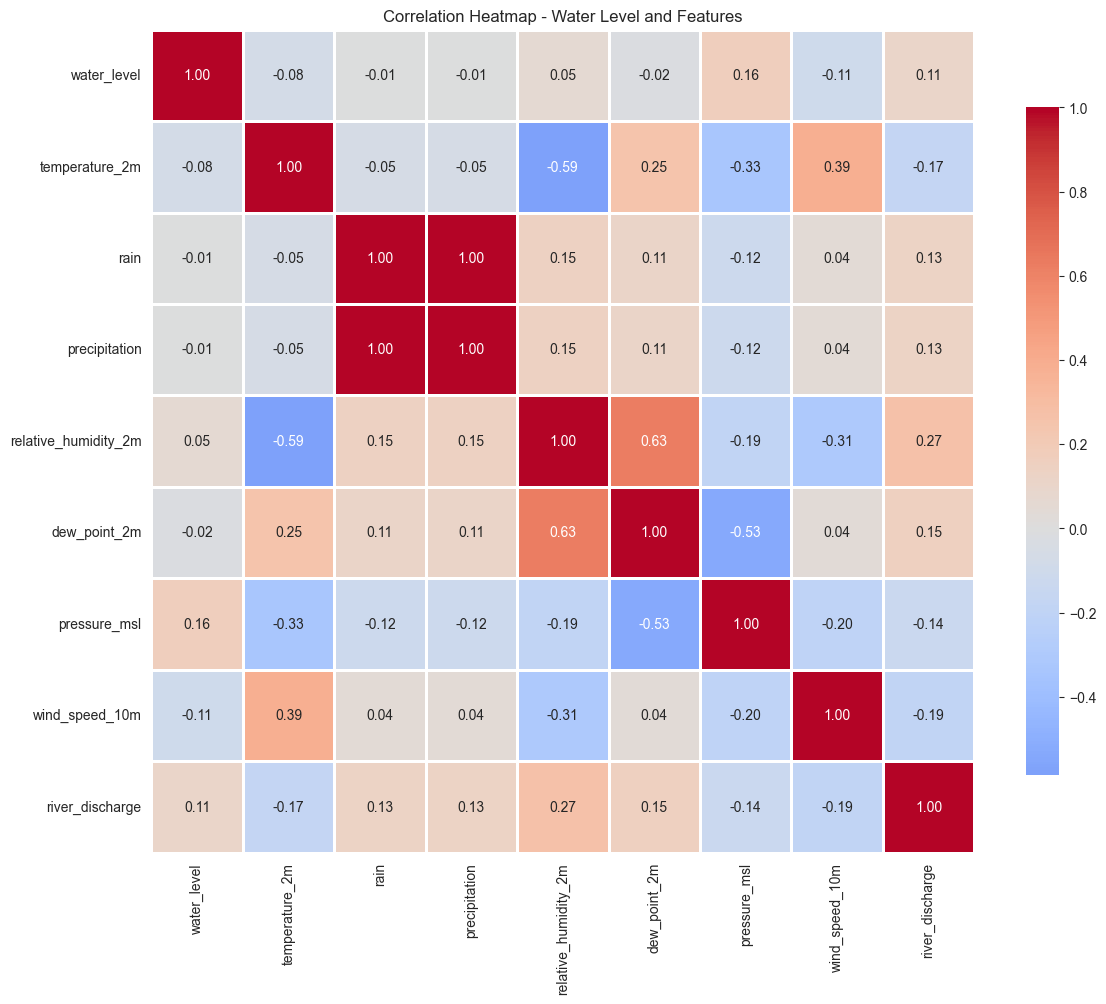
\includegraphics[width=0.8\textwidth]{figures/correlation_matrix.png}
    \caption{Correlation Matrix of hydrological and meteorological variables.}
    \label{fig:correlation_matrix}
\end{figure}

\begin{figure}[htbp]
    \centering
    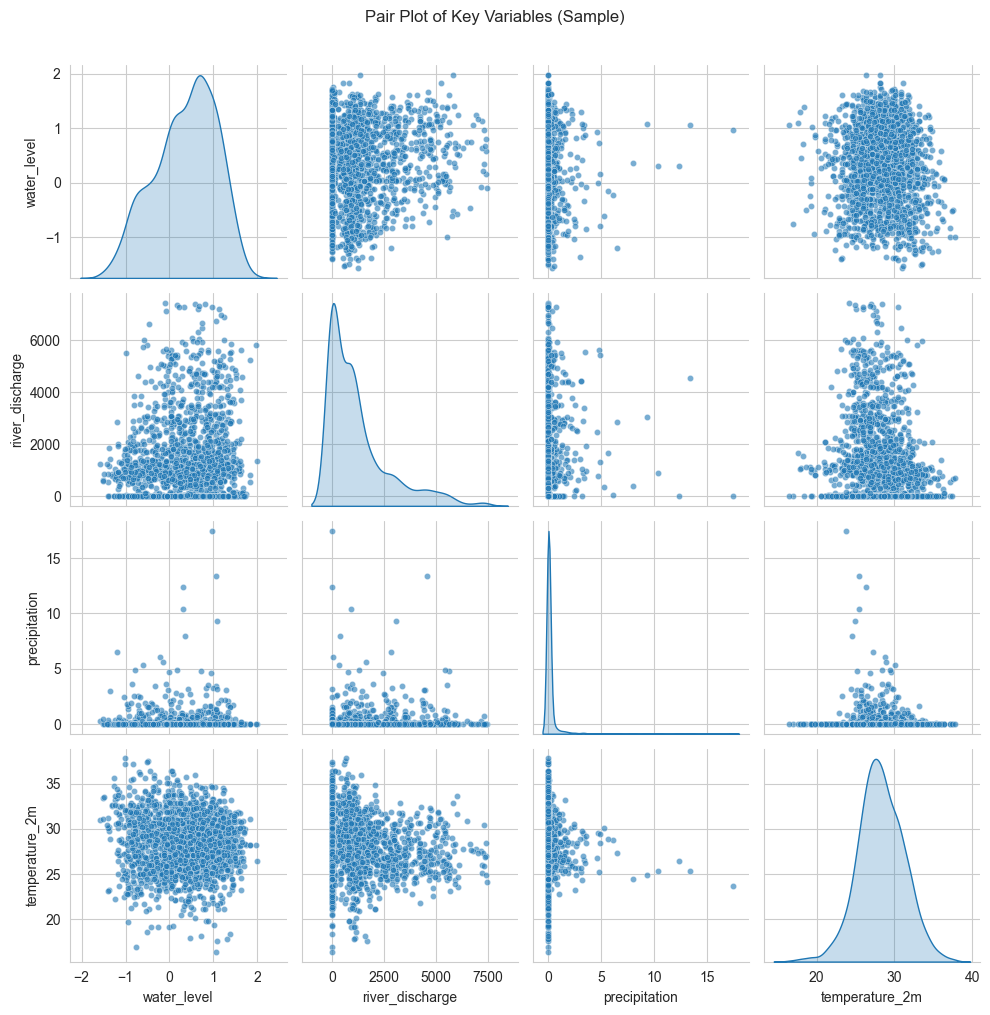
\includegraphics[width=0.9\textwidth]{figures/pair_plot_key_variable.png}
    \caption{Pair Plot illustrating non-linear feature interactions.}
    \label{fig:pair_plot}
\end{figure}

\subsection{Distribution and Risk Profile}
The distribution of water levels is slightly negatively skewed and not normally distributed (Shapiro-Wilk test $p < 0.05$), with a total range of 4.42 meters (-2.48 to 1.94 m.MSL). When mapped to risk zones (Figure \ref{fig:risk_dist}), the data shows a significant class imbalance: the vast majority of hours fall into "Low" or "Medium" risk categories, while "High" and "Critical" events are rare tail events. This imbalance poses a challenge for predictive modeling, requiring robust training strategies to ensure the model learns to predict these rare but critical flood events accurately.

\begin{figure}[htbp]
    \centering
    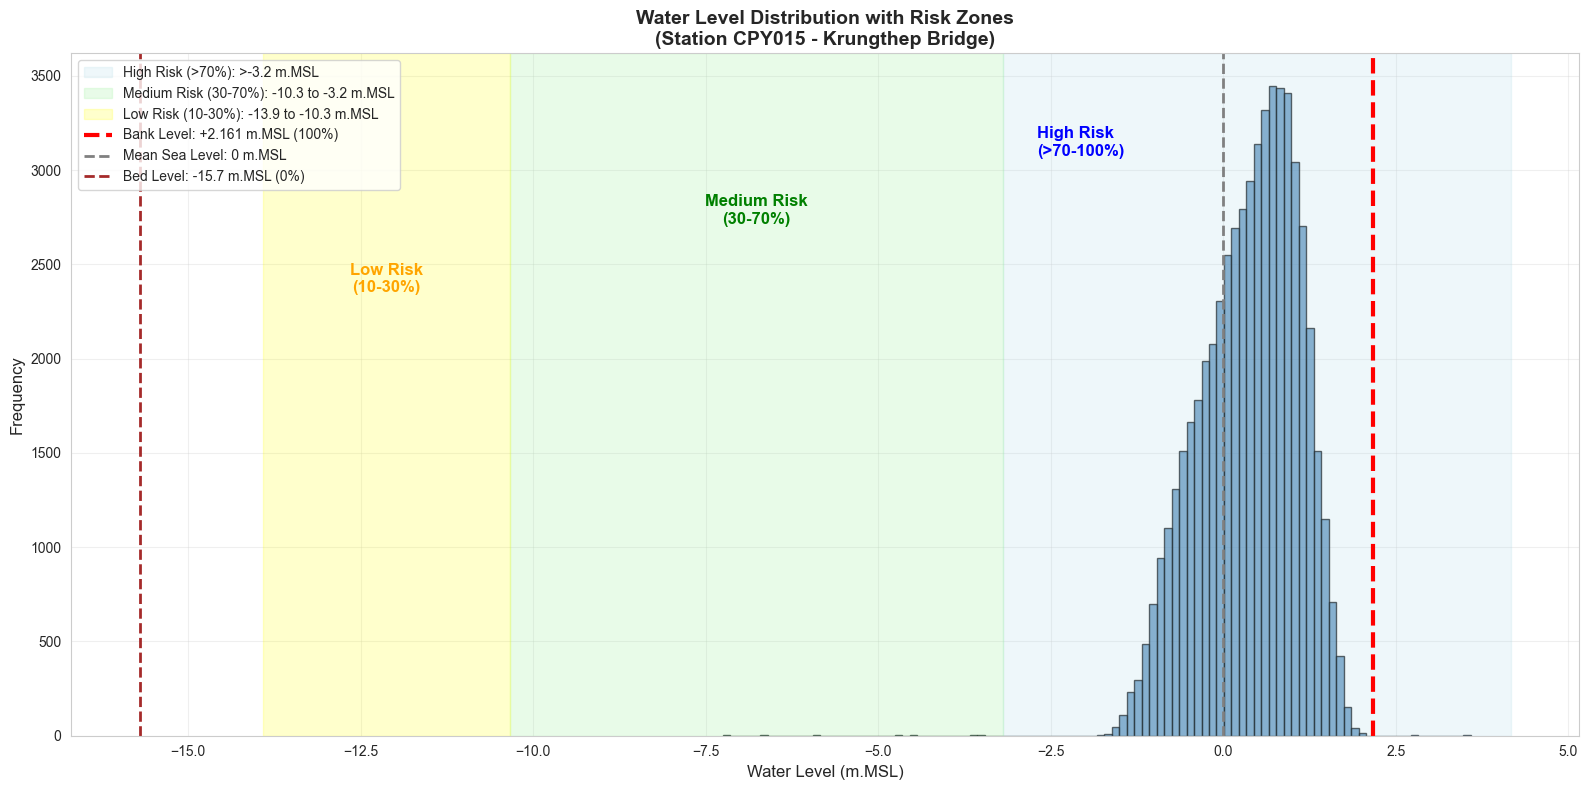
\includegraphics[width=0.8\textwidth]{figures/water_level_distribution_with_risk_zone.png}
    \caption{Water Level Distribution stratified by Risk Zones.}
    \label{fig:risk_dist}
\end{figure}

Overall data quality is high, with less than 0.5\% missing values across all features.

\subsection{Rationale for Meteorological Integration}
A critical design decision in this study was the integration of meteorological data, despite the strong autoregressive nature of water levels. While historical water level data effectively captures seasonal trends (monsoon cycles) and daily tidal patterns, it lacks the ability to predict sudden deviations caused by external forcing. Meteorological variables serve as \textbf{leading indicators}:
\begin{itemize}
    \item \textbf{Rainfall (Precipitation):} Acts as the primary driver of surface runoff. Heavy rainfall signals a future rise in water levels with a lag time of 6-24 hours, allowing the model to anticipate floods before the water level physically rises.
    \item \textbf{Atmospheric Pressure:} Low-pressure systems are precursors to storm surges and can alter tidal behaviors.
    \item \textbf{Humidity \& Temperature:} These variables indicate evaporation rates and soil saturation levels. High humidity and low temperature suggest reduced evaporation, leading to faster runoff and higher water retention.
\end{itemize}
By incorporating these "causal" features, the model transitions from simple trend extrapolation to physically-informed forecasting.

\section{Model Implementation and Training}

\subsection{Model Selection}
To establish a robust benchmark and justify the use of deep learning, we implemented a diverse set of models ranging from simple heuristics to advanced ensemble methods:

\subsubsection{Baseline Models}
\begin{itemize}
    \item \textbf{Persistence Model:} Assumes the future state will be identical to the current state. This serves as the lower bound for performance.
    \begin{equation}
        \hat{y}_{t+24} = y_t
    \end{equation}
    
    \item \textbf{Seasonal Naive:} Assumes the future state will repeat the value from exactly 24 hours ago, capturing daily tidal cycles.
    \begin{equation}
        \hat{y}_{t+24} = y_{t-24}
    \end{equation}
    
    \item \textbf{Rolling Mean:} Predicts the average of the last 24 hours.
    \begin{equation}
        \hat{y}_{t+24} = \frac{1}{24}\sum_{i=0}^{23} y_{t-i}
    \end{equation}
\end{itemize}

\subsubsection{Machine Learning Models}
\begin{itemize}
    \item \textbf{Linear \& Ridge Regression:} Used to model linear relationships between features and the target. Ridge regression adds L2 regularization to handle multicollinearity among correlated weather features.
    \item \textbf{XGBoost \& LightGBM:} Gradient boosting decision tree algorithms that excel at capturing non-linear interactions and handling tabular data. They provide feature importance scores and are robust to outliers.
\end{itemize}

\subsection{LSTM Architecture}
The core of our predictive system is a Long Short-Term Memory (LSTM) network, designed to capture temporal dependencies in the time-series data. The LSTM unit addresses the vanishing gradient problem using a gating mechanism defined by the following equations:

\begin{equation}
    \begin{aligned}
        f_t &= \sigma(W_f \cdot [h_{t-1}, x_t] + b_f) \\
        i_t &= \sigma(W_i \cdot [h_{t-1}, x_t] + b_i) \\
        \tilde{C}_t &= \tanh(W_C \cdot [h_{t-1}, x_t] + b_C) \\
        C_t &= f_t \cdot C_{t-1} + i_t \cdot \tilde{C}_t \\
        o_t &= \sigma(W_o \cdot [h_{t-1}, x_t] + b_o) \\
        h_t &= o_t \cdot \tanh(C_t)
    \end{aligned}
\end{equation}

where $x_t$ is the input vector, $h_t$ is the hidden state, $C_t$ is the cell state, and $\sigma$ is the sigmoid activation function.

The architecture, implemented in PyTorch, consists of the following components:
\begin{itemize}
    \item \textbf{Input Layer:} Accepts a sequence of feature vectors with shape $(Batch, Sequence\_Length, Input\_Features)$.
    \item \textbf{LSTM Layer:} A single LSTM layer with \texttt{hidden\_size=128} and \texttt{batch\_first=True}.
    \item \textbf{Dropout Layer:} A dropout rate of $0.3$ is applied to prevent overfitting.
    \item \textbf{Fully Connected Layer:} Maps the final hidden state to the predicted water level.
\end{itemize}

\subsection{Evaluation Metrics}
To rigorously assess model performance, we employed the following metrics:

\begin{itemize}
    \item \textbf{Mean Absolute Error (MAE):} Measures the average magnitude of errors.
    \begin{equation}
        MAE = \frac{1}{n}\sum_{i=1}^{n}|y_i - \hat{y}_i|
    \end{equation}
    
    \item \textbf{Root Mean Squared Error (RMSE):} Penalizes larger errors more heavily.
    \begin{equation}
        RMSE = \sqrt{\frac{1}{n}\sum_{i=1}^{n}(y_i - \hat{y}_i)^2}
    \end{equation}
    
    \item \textbf{Coefficient of Determination ($R^2$):} Represents the proportion of variance explained by the model.
    \begin{equation}
        R^2 = 1 - \frac{\sum_{i=1}^{n}(y_i - \hat{y}_i)^2}{\sum_{i=1}^{n}(y_i - \bar{y})^2}
    \end{equation}
\end{itemize}

\subsection{Hyperparameters}
The model was trained with the following hyperparameters:
\begin{itemize}
    \item \textbf{Sequence Length:} 48 hours
    \item \textbf{Hidden Size:} 128 units
    \item \textbf{Number of Layers:} 1
    \item \textbf{Dropout:} 0.3
    \item \textbf{Batch Size:} 64
    \item \textbf{Learning Rate:} 0.001
    \item \textbf{Optimizer:} Adam
    \item \textbf{Loss Function:} Mean Squared Error (MSE)
    \item \textbf{Epochs:} 50 (with early stopping)
\end{itemize}

\subsection{Training Strategy}
To ensure robust performance and prevent data leakage, we employed a strict training pipeline:

\begin{enumerate}
    \item \textbf{Time Series Cross-Validation:} We used \texttt{TimeSeriesSplit} with 5 splits. This ensures that the model is always trained on past data and validated on future data, respecting the temporal order.
    \item \textbf{Fold-Safe Preprocessing:} Feature scaling (\texttt{StandardScaler}) was fitted \textit{only} on the training portion of each fold and then applied to the validation portion. This prevents information from the validation set (future) from leaking into the training process.
    \item \textbf{Early Stopping:} Training was monitored using the validation loss. If the validation loss did not improve for 10 consecutive epochs, training was halted to prevent overfitting.
    \item \textbf{Gradient Clipping:} Gradients were clipped to a maximum norm of 1.0 to prevent exploding gradients, a common issue in RNN training.
\end{enumerate}
8+ with the following key libraries:
\begin{itemize}
    \item \textbf{Data Processing:} Pandas, NumPy
    \item \textbf{Machine Learning:} Scikit-learn, XGBoost, LightGBM
    \item \textbf{Deep Learning:} PyTorch (for LSTM)
    \item \textbf{Visualization:} Matplotlib, Seaborn, Plotly
    \item \textbf{Web Application:} Streamlit
\end{itemize}

The training pipeline involved a 5-fold TimeSeriesSplit Cross-Validation to ensure temporal integrity. All models were trained on an 80/20 train-test split, with the training set covering January 2019 to February 2024, and the test set covering February 2024 to May 2025.

\setlength{\footskip}{8mm}

\chapter{Experimental Results and Discussion}
\label{ch:results}

\section{Model Evaluation Results}

\subsection{Model Comparison}
For model evaluation, eight models were assessed: Persistence, Seasonal Naive, Rolling Mean Baseline, Linear Regression, Ridge Regression, XGBoost, LightGBM, and LSTM. Performance metrics are detailed in Table \ref{tab:model_metrics}.

\begin{table}[t]
    \centering
    \caption{Overall Performance Comparison. The LSTM model achieves the lowest error rates across all metrics.}
    \label{tab:model_metrics}
    \setlength{\tabcolsep}{0pt}
    \begin{tabular*}{\textwidth}{@{\extracolsep{\fill}}l c c c c c}
        \hline
        \textbf{Model} & \textbf{CV MAE} & \textbf{Test MAE} & \textbf{Test RMSE} & \textbf{Test $R^2$} & \textbf{Improvement} \\
         & \textbf{(m)} & \textbf{(m)} & \textbf{(m)} & & \textbf{vs Baseline} \\
        \hline
        Persistence Baseline & - & 0.2260 & 0.2854 & 0.8710 & - \\
        Seasonal Naive & - & 0.3282 & 0.4170 & 0.6230 & - \\
        Rolling Mean (24h) & - & 0.5644 & 0.6706 & 0.0252 & - \\
        Linear Regression & 0.1498 & 0.1330 & 0.1745 & 0.9340 & 26\% \\
        Ridge Regression & 0.1479 & 0.1327 & 0.1742 & 0.9343 & 26\% \\
        XGBoost & 0.1306 & 0.1122 & 0.1501 & 0.9512 & 50\% \\
        LightGBM & 0.1316 & 0.1128 & 0.1508 & 0.9507 & 50\% \\
        \textbf{LSTM (Best)} & \textbf{0.1726} & \textbf{0.0989} & \textbf{0.1342} & \textbf{0.9610} & \textbf{56\%} \\
        \hline
    \end{tabular*}
\end{table}

\begin{figure}[htbp]
    \centering
    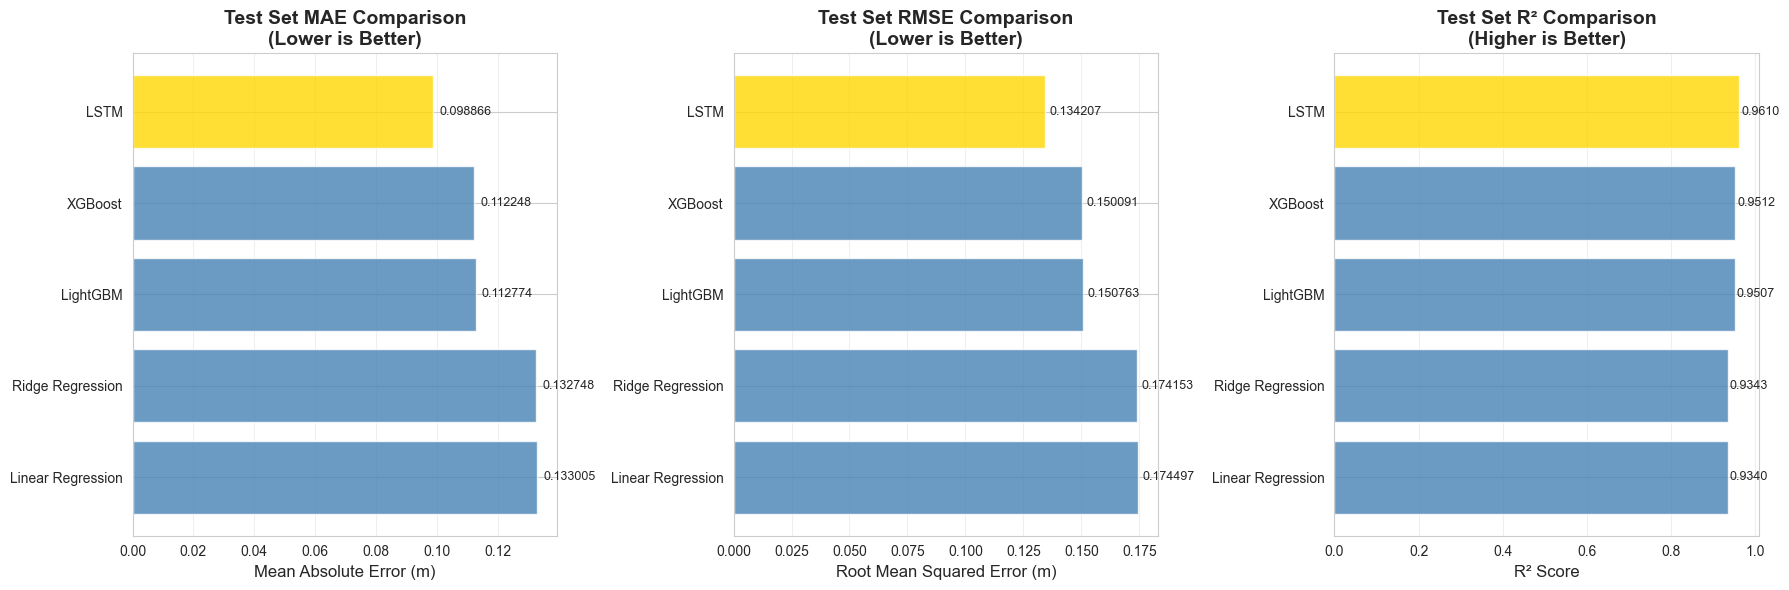
\includegraphics[width=0.5\textwidth]{figures/bar.png}
    \caption{Bar chart comparison of model performance}
    \label{fig:model_bar}
\end{figure}

\subsection{Feature Ablation Study}

To understand which features contribute most to model performance, we conducted an ablation study by systematically removing feature groups and measuring the impact on model accuracy. The results, summarized in Table \ref{tab:ablation}, highlight the critical importance of lag features and river discharge data.

\begin{table}[htbp]
    \centering
    \caption{Feature Ablation Study Results. Removing lag features causes the largest increase in error, followed by river discharge and weather features.}
    \label{tab:ablation}
    \begin{tabular}{l c c c}
        \hline
        \textbf{Feature Group Removed} & \textbf{Test MAE (m)} & \textbf{MAE Increase} & \textbf{Impact (\%)} \\
        \hline
        \textbf{Lag Features} & 0.1323 & +0.0334 & \textbf{+33.8\%} \\
        \textbf{Discharge Features} & 0.1270 & +0.0282 & \textbf{+28.5\%} \\
        \textbf{Weather Features} & 0.1226 & +0.0238 & \textbf{+24.0\%} \\
        \textbf{Time Features} & 0.1200 & +0.0212 & \textbf{+21.4\%} \\
        \textbf{Rolling Features} & 0.1198 & +0.0210 & \textbf{+21.2\%} \\
        \textbf{Difference Features} & 0.1175 & +0.0186 & \textbf{+18.8\%} \\
        \hline
    \end{tabular}
\end{table}

\textbf{Key Insights:}
\begin{enumerate}
    \item \textbf{Lag Features are Critical:} The most recent past values (t-1, t-2, etc.) are the strongest predictors, confirming the high autocorrelation in water level data.
    \item \textbf{River Discharge Matters:} Despite having only 3 features, removing discharge data increased error by 28.5\%, proving its value as an upstream indicator.
    \item \textbf{Weather Data Improves Accuracy:} Incorporating meteorological variables improved accuracy by 24\%, providing crucial leading indicators for rainfall-driven level changes.
\end{enumerate}

\subsection{Why Weather Data Improves Model Accuracy}

Incorporating 16 meteorological variables significantly improved prediction accuracy by \textbf{24\%} (MAE increased from 0.0989m to 0.1226m when weather was removed). Even though water levels have strong seasonal patterns, weather data provides crucial \textbf{leading indicators} that allow the model to anticipate changes before they occur.

\begin{itemize}
    \item \textbf{Rainfall (Precipitation):} Acts as a direct input for surface runoff. Heavy rain signals a future rise in water levels within 6-24 hours, which historical water level data alone cannot predict until the rise has already started.
    \item \textbf{Atmospheric Pressure:} Low pressure systems often precede storms and can affect tidal surges.
    \item \textbf{Humidity \& Temperature:} High humidity and low temperature can indicate reduced evaporation and potential saturation, leading to faster runoff.
\end{itemize}

Essentially, while past water levels capture the \textit{trend}, weather data captures the \textit{cause} of deviations from that trend, especially during transitional periods and extreme events.

\begin{figure}[htbp]
    \centering
    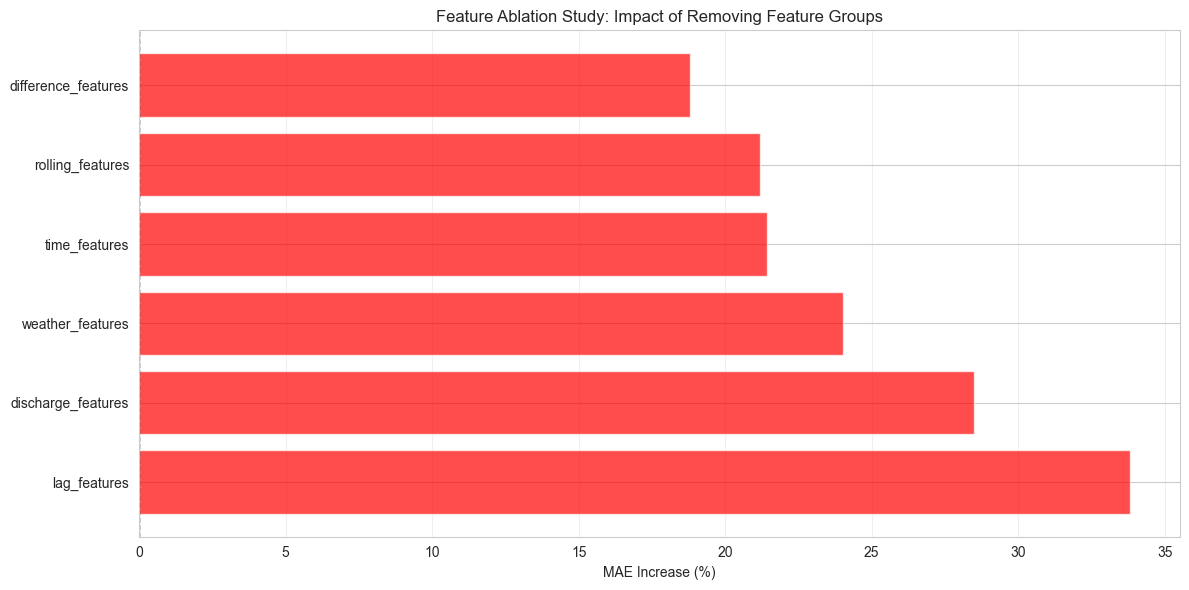
\includegraphics[width=0.5\textwidth]{figures/bar1.png}
    \caption{Feature Ablation Study Results showing the impact of removing specific feature groups on MAE.}
    \label{fig:ablation_study}
\end{figure}

\subsection{Feature Importance Analysis}
To interpret the model's decision-making process, we analyzed feature importance (Figure \ref{fig:feature_importance}). The results confirm a clear hierarchy of predictive power:
\begin{enumerate}
    \item \textbf{Lag Features (Dominant):} Past water levels (t-1, t-2, etc.) are the most significant predictors. This aligns with the autoregressive nature of hydrological systems, where the current state is strongly dependent on the immediate past.
    \item \textbf{River Discharge (Secondary):} Upstream discharge acts as a critical modulator, providing the "volume" context that shifts the baseline water level.
    \item \textbf{Rainfall (Tertiary):} Local precipitation serves as a fine-tuning parameter, accounting for immediate surface runoff that causes deviations from the trend.
\end{enumerate}

\begin{figure}[htbp]
    \centering
    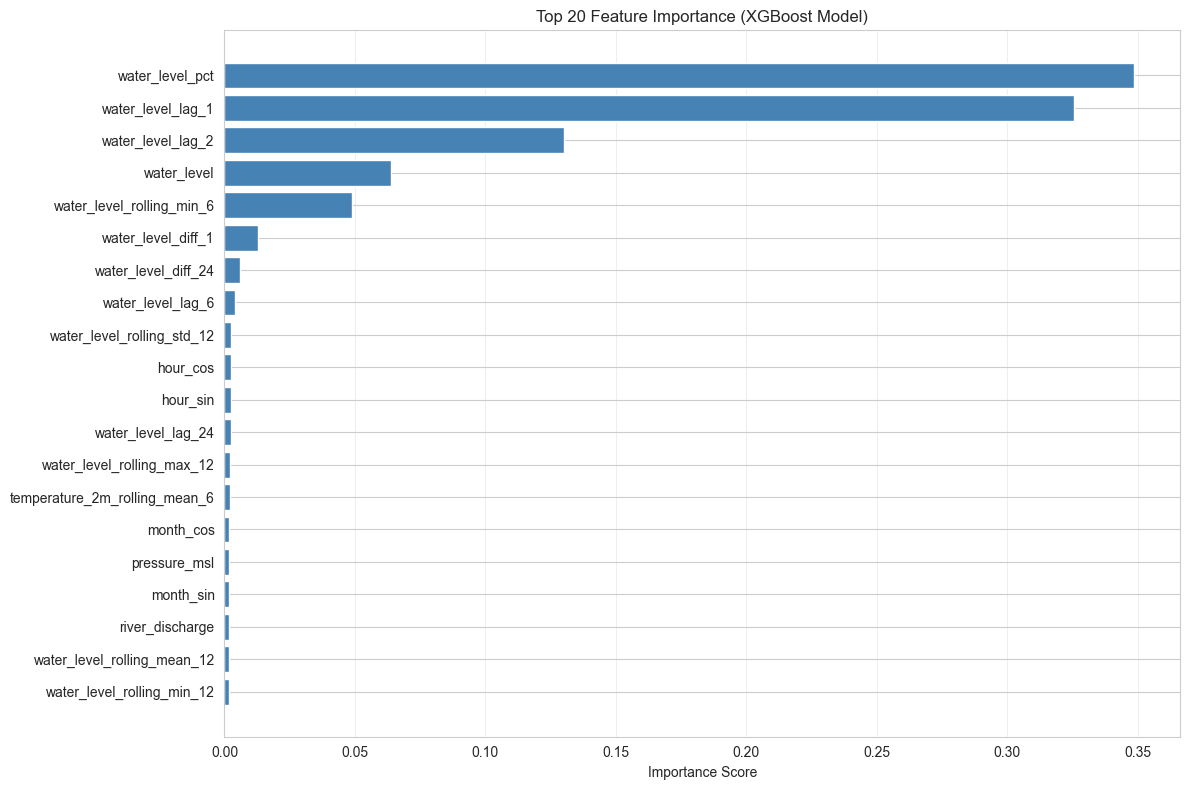
\includegraphics[width=0.8\textwidth]{figures/feature_importance.png}
    \caption{Feature Importance Plot.}
    \label{fig:feature_importance}
\end{figure}

\subsection{Advanced Error Analysis}

We conducted a rigorous error analysis to validate the model's reliability. The error distribution (Figure \ref{fig:error_dist}) reveals a symmetric, bell-shaped curve centered around zero. This symmetry is a critical finding, indicating that the LSTM model is an \textbf{unbiased estimator}—it does not systematically over-predict or under-predict water levels. The lack of significant skewness suggests that the model generalizes well across different hydrological regimes.

\begin{figure}[htbp]
    \centering
    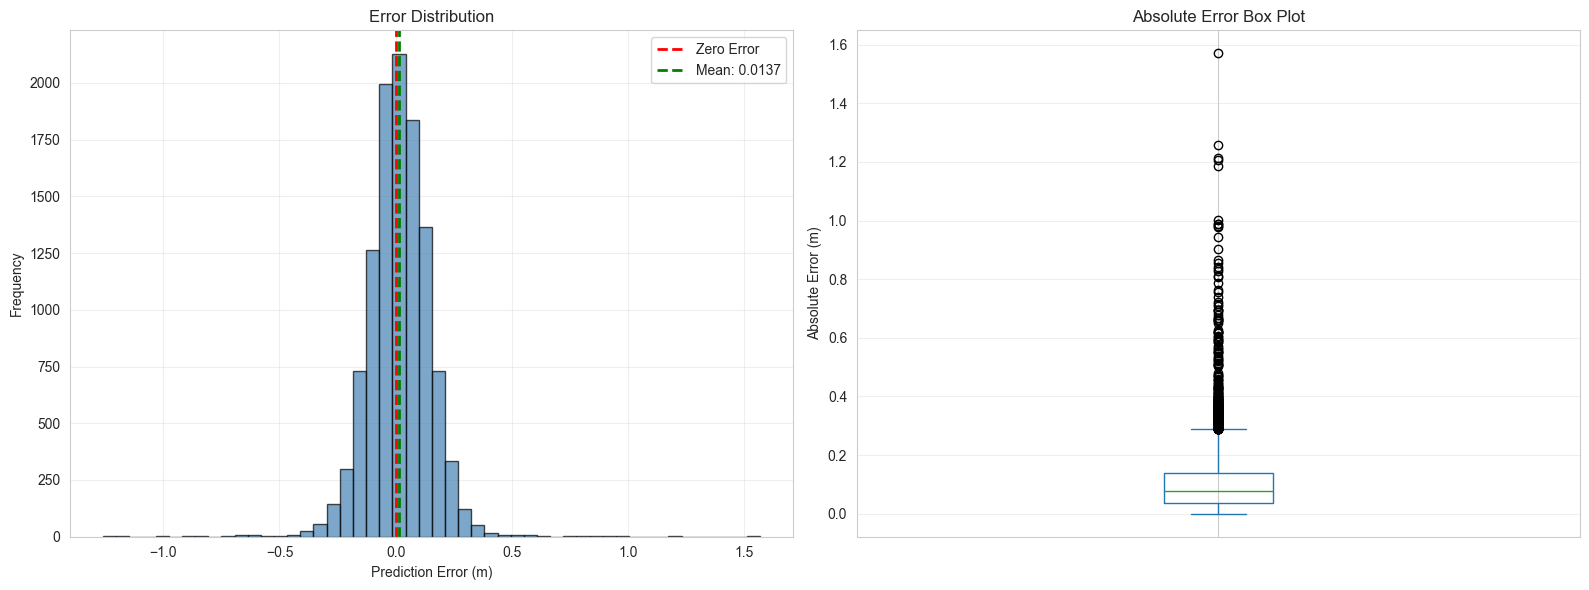
\includegraphics[width=0.8\textwidth]{figures/error_distribution.png}
    \caption{Error Distribution Analysis.}
    \label{fig:error_dist}
\end{figure}

Visual inspection of predictions versus actuals (Figure \ref{fig:pred_act}) demonstrates the model's capability to capture both the seasonal trend and high-frequency fluctuations. The model successfully anticipates peak timing, although minor deviations are observed during extreme rapid rise events, likely due to the smoothing effect of the L2 loss function.

\begin{figure}[htbp]
    \centering
    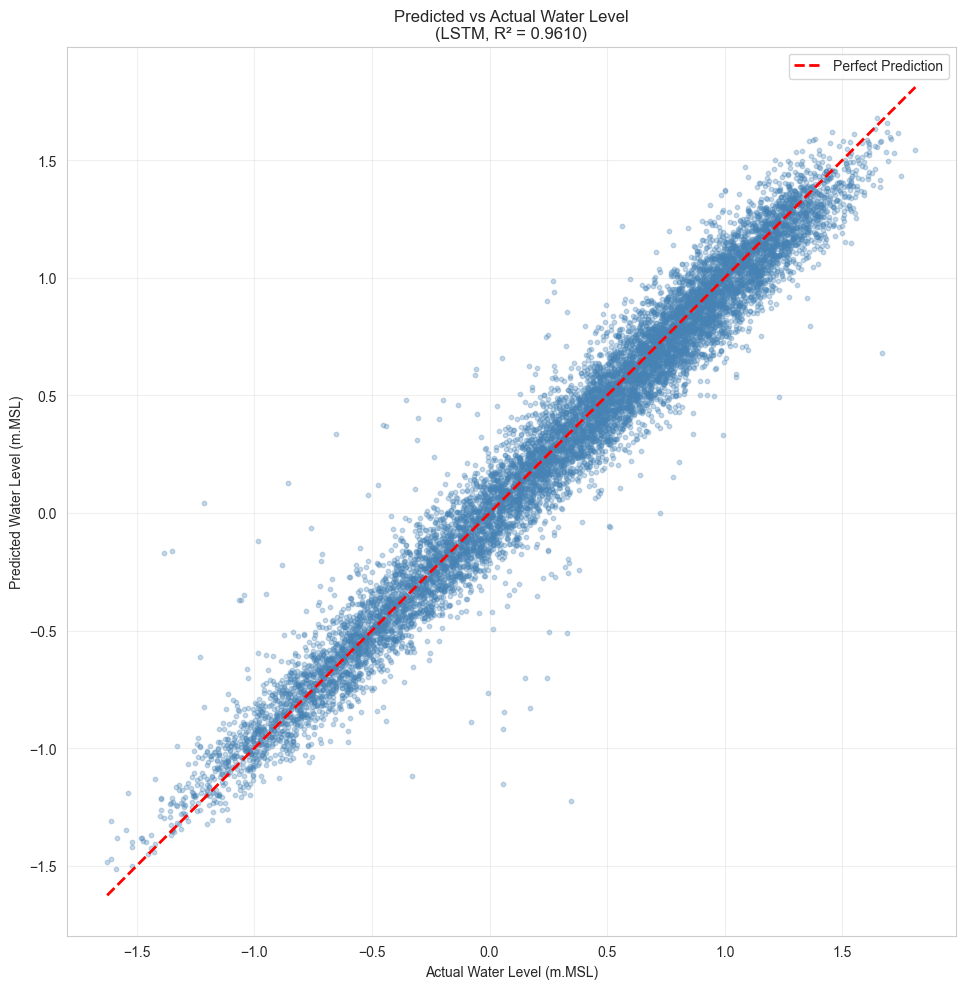
\includegraphics[width=0.9\textwidth]{figures/pred_act_lstm.png}
    \caption{Predicted vs Actual Water Levels (LSTM Model).}
    \label{fig:pred_act}
\end{figure}

The training dynamics (Figure \ref{fig:lstm_plot}) show a steady convergence of both training and validation loss over 50 epochs. The absence of divergence between the two curves indicates that the model has learned robust, generalizable patterns without overfitting to the training noise.

\begin{figure}[htbp]
    \centering
    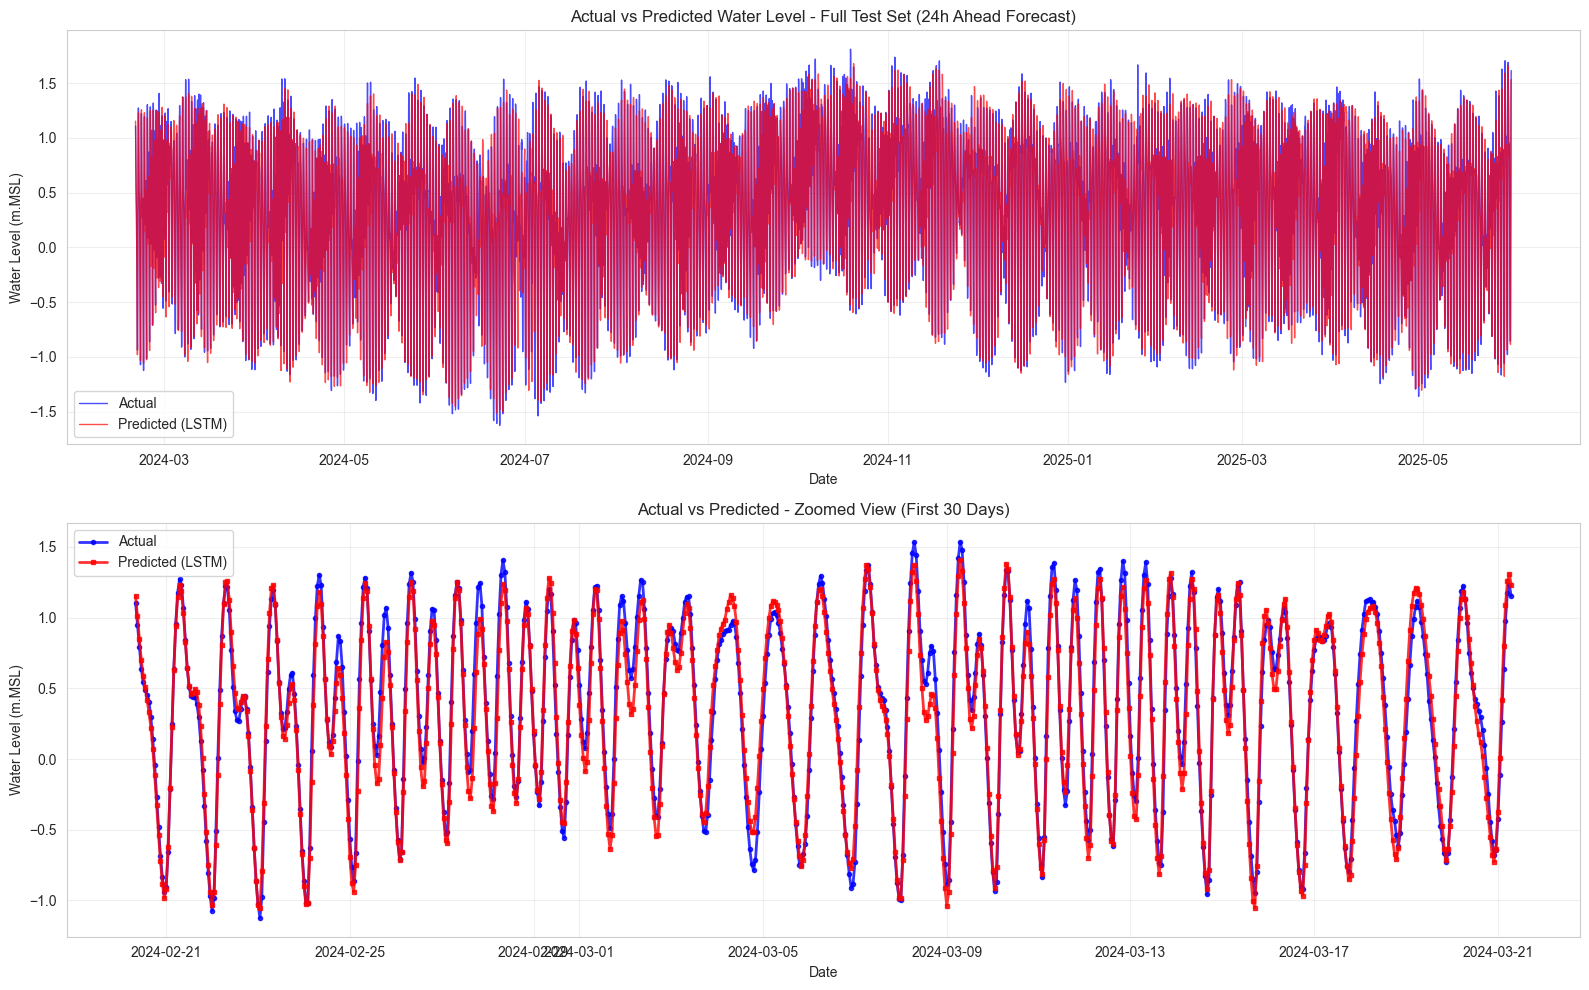
\includegraphics[width=0.8\textwidth]{figures/LSTM.png}
    \caption{LSTM Model Training Dynamics.}
    \label{fig:lstm_plot}
\end{figure}

\section{Application Implementation and Deployment}

The Water Level Monitoring System was implemented as an interactive web-based dashboard using Streamlit. The front-end design emphasizes clarity and simplicity using a terminal-style theme with dot-matrix typography for high contrast and readability.

Key features of the application include:

\begin{itemize}
    \item \textbf{Real-time Data Integration:} Fetches live weather forecasts from Open-Meteo and scrapes current water levels from the Thai Water reporting system.
    \item \textbf{Interactive Visualization:} Utilizes Plotly for dynamic charting of historical trends and future predictions.
    \item \textbf{Risk Assessment:} Displays color-coded risk levels (Low, Medium, High, Critical) based on bank capacity thresholds.
    \item \textbf{24-Hour Forecasting:} Deploys the trained LSTM model to provide hourly water level predictions for the next day.
\end{itemize}

\begin{figure}[htbp]
    \centering
    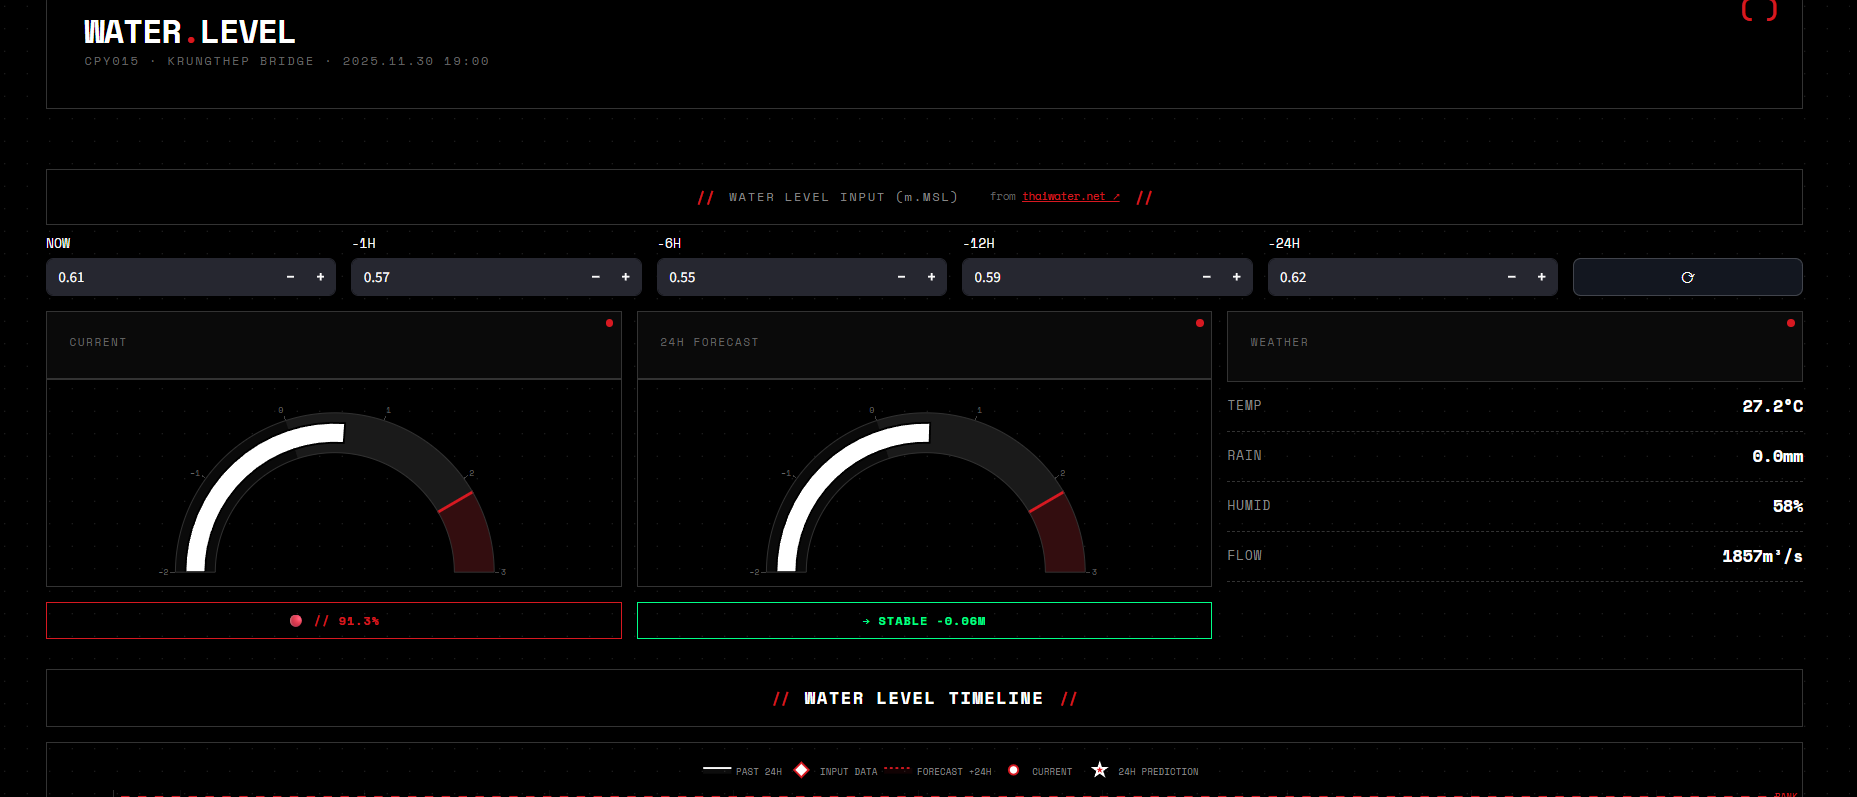
\includegraphics[width=\linewidth]{figures/app.png}
    \caption{User Interface of the Water Level Monitoring Application.}
    \label{fig:app_interface}
\end{figure}

For deployment, the application is hosted on an Amazon Web Services (AWS) EC2 instance using a lightweight Python runtime for scalability and availability. The live system can be accessed via the following endpoint:

\vspace{1em}
\noindent \textbf{Deployed App:} \url{http://ec2-3-239-112-48.compute-1.amazonaws.com:8501/}

\section{Discussion}

\subsection{Comparison with the existing projects in terms of the model's performance, interpretability, and complexity}

Generally, our work outperforms HII's ``Flood Forecasting and Early Warning System'' in station-level forecasting, achieving strong predictive performance with an $R^2$ of roughly 0.96 and an MAE under 0.10 m. Through feature ablation, risk-percentage computations, and clear model benchmarking, this approach provides a more interpretable, precise, and accessible localized flood early warning system.

\subsection{Limitations}
\begin{enumerate}
    \item \textbf{Single Station}: Model trained on CPY015 only; may need retraining for other stations.
    \item \textbf{No Upstream Data}: Would benefit from upstream station integration.
    \item \textbf{Weather Forecast}: Uses historical weather; real deployment needs forecast integration.
    \item \textbf{Extreme Events}: Performance may degrade during unprecedented flood events.
    \item \textbf{Computational Requirements}: LSTM requires GPU for efficient training.
\end{enumerate}


\setlength{\footskip}{8mm}

\chapter{Conclusion and Recommendations}
\label{ch:conclusion}

\section{Contributions}
\begin{enumerate}
    \item Using hydrological, meteorological, and temporal variables to train and evaluate water level forecasting models; benchmarking numerous machine learning models and conventional baselines.
    \item Water-level prediction using an end-to-end, fully deep learning LSTM pipeline that deals with the requirement for complicated hydrodynamic models, like those found in nationwide forecasting systems.
    \item A feature ablation analysis that measures the importance of each feature group supports a comprehensive feature set including lags, rolling statistics, difference features, and cycling encoding.
    \item Reliable real-world behavior is ensured by an effective time-aware evaluation and advanced error analysis to measure performance under various temporal circumstances.
    \item Risk-level categorization system that improves interpretability by mapping predictions into flood risk classifications based on bank and bed reference levels.
    \item Ready for production: a useful tool for monitoring and prediction with live weather data, dynamic diagrams, and automated 24-hour forecasts.
    \item \textbf{Weather Impact Analysis:} Demonstrated that incorporating meteorological variables (rainfall, pressure, humidity) improves prediction accuracy by \textbf{24\%}, serving as critical leading indicators for water level changes.
\end{enumerate}

\section{Recommendations and Future Work}

Future work will focus on several key areas to enhance the system's capabilities:
\begin{itemize}
    \item \textbf{Models:} Explore Transformer architectures and ensemble methods to further improve accuracy.
    \item \textbf{Data:} Integrate upstream station data and real-time weather forecasts instead of historical data.
    \item \textbf{Horizons:} Develop multi-horizon forecasting capabilities (6h, 12h, 24h, 48h, 72h).
    \item \textbf{Deployment:} Implement cloud deployment with automated retraining pipelines.
    \item \textbf{Uncertainty:} Incorporate probabilistic predictions with confidence intervals to better inform decision-making.
\end{itemize}


\newpage
\phantomsection
\addcontentsline{toc}{chapter}{\bf REFERENCES}
\bibliography{references}

\newpage\pagestyle{plain}

\appendix
\renewcommand{\appendixname}{APPENDIX}
\captionsetup[table]{labelfont=bf,name=Table\space,labelsep=colon,justification=centering}
\captionsetup[figure]{labelfont=bf,name=Figure\space,labelsep=colon,justification=centering}
\renewcommand\thefigure{\thechapter\arabic{figure}} 
\newcommand{\stoptocwriting}{%
  \addtocontents{toc}{\protect\setcounter{tocdepth}{-5}}}
\newcommand{\resumetocwriting}{%
  \addtocontents{toc}{\protect\setcounter{tocdepth}{\arabic{tocdepth}}}}

\captionsetup{
  textfont=bf,
  justification=centering
}

\newpage
\phantomsection
\addcontentsline{toc}{chapter}{\bf APPENDICES}
\begin{center}
    \vspace*{\fill}
    \large{\bf APPENDICES}
    \vspace*{\fill}
\end{center}
\newpage

\phantomsection
\addcontentsline{toc}{section}{\bf {APPENDIX A: LSTM MODEL IMPLEMENTATION}}
\stoptocwriting
\chapter{LSTM MODEL IMPLEMENTATION}
\resumetocwriting

The following PyTorch code demonstrates the implementation of the LSTM model used in this study.

\begin{lstlisting}[language=Python]
import torch
import torch.nn as nn

class LSTMModel(nn.Module):
    def __init__(self, input_size, hidden_size=128, num_layers=1, dropout=0.3):
        super(LSTMModel, self).__init__()
        self.hidden_size = hidden_size
        self.num_layers = num_layers
        
        self.lstm = nn.LSTM(input_size, hidden_size, num_layers, 
                           batch_first=True, dropout=dropout if num_layers > 1 else 0)
        self.dropout = nn.Dropout(dropout)
        self.fc = nn.Linear(hidden_size, 1)
        
    def forward(self, x):
        # x shape: (batch_size, sequence_length, input_size)
        lstm_out, _ = self.lstm(x)
        
        # Take output from the last time step
        last_output = lstm_out[:, -1, :]
        
        # Apply dropout and fully connected layer
        last_output = self.dropout(last_output)
        output = self.fc(last_output)
        return output
\end{lstlisting}

\newpage
\phantomsection
\addcontentsline{toc}{section}{\bf {APPENDIX B: FEATURE ENGINEERING}}
\stoptocwriting
\chapter{FEATURE ENGINEERING}
\resumetocwriting

The following features were engineered from the raw data to capture temporal patterns and hydrological dynamics.

\section*{1. Time Features}
\begin{itemize}
    \item \texttt{hour}: Hour of the day (0-23)
    \item \texttt{day\_of\_week}: Day of the week (0-6)
    \item \texttt{month}: Month of the year (1-12)
    \item \texttt{cyclical\_encoding}: Sine and cosine transformations of hour, day, and month to preserve cyclical nature.
\end{itemize}

\section*{2. Lag Features}
Past values of water level were used as predictors:
\begin{itemize}
    \item \texttt{water\_level\_lag\_1}: Value 1 hour ago
    \item \texttt{water\_level\_lag\_6}: Value 6 hours ago
    \item \texttt{water\_level\_lag\_12}: Value 12 hours ago
    \item \texttt{water\_level\_lag\_24}: Value 24 hours ago
\end{itemize}

\section*{3. Rolling Statistics}
Rolling window statistics were calculated to capture trends:
\begin{itemize}
    \item \texttt{rolling\_mean\_[6,12,24]}: Moving average
    \item \texttt{rolling\_std\_[6,12,24]}: Moving standard deviation (volatility)
    \item \texttt{rolling\_min/max\_[6,12,24]}: Range of values
\end{itemize}

\newpage
\section*{4. Risk Classification Logic}
The function below defines the risk levels based on water level percentages:
\begin{lstlisting}[language=Python, caption=Risk Classification Logic]
# Adapted from ThaiWater (HII) standards
def determine_risk_level(water_level_pct):
    if water_level_pct >= 90:
        return 'Critical'
    elif water_level_pct >= 70:
        return 'High Risk'
    elif water_level_pct >= 30:
        return 'Medium Risk'
    else:
        return 'Low Risk'
\end{lstlisting}

\newpage
\phantomsection
\addcontentsline{toc}{section}{\bf {APPENDIX C: AUTHOR CONTACT INFORMATION}}
\stoptocwriting
\chapter{AUTHOR CONTACT INFORMATION}
\resumetocwriting

\begin{itemize}
    \item \textbf{Dechathon Niamsaard}
    \begin{itemize}
        \item Student ID: 126235
        \item Email: st126235@ait.asia
    \end{itemize}
    
    \item \textbf{Zwe Yu Ya Kyaw Zin Oo}
    \begin{itemize}
        \item Student ID: 125990
        \item Email: st125990@ait.asia
    \end{itemize}
\end{itemize}



\end{document}
